\documentclass[aspectratio=169,11pt]{beamer}
\usepackage[T1]{fontenc}
\usepackage[utf8]{inputenc}
\usepackage{lmodern}
\usepackage{amsmath,amssymb,mathtools,booktabs,array}
\usepackage{tikz}
\usetikzlibrary{arrows.meta,positioning,calc}
\usepackage{ragged2e}
\usepackage{microtype}
\definecolor{Navy}{HTML}{162D45}
\definecolor{Petrol}{HTML}{176C75}
\definecolor{Ink}{HTML}{25384B}
\definecolor{Muted}{HTML}{61768A}
\definecolor{Bg}{HTML}{F7F9FB}
\definecolor{Pale}{HTML}{E7F0F2}
\definecolor{Line}{HTML}{DCE5ED}
\setbeamercolor{normal text}{fg=Ink,bg=white}
\setbeamercolor{structure}{fg=Petrol}
\setbeamercolor{frametitle}{fg=Navy,bg=white}
\setbeamercolor{title}{fg=Navy}
\setbeamercolor{subtitle}{fg=Muted}
\setbeamercolor{block title}{bg=Petrol,fg=white}
\setbeamercolor{block body}{bg=Pale,fg=Ink}
\setbeamercolor{alerted text}{fg=Petrol}
\setbeamercolor{item}{fg=Petrol}
\setbeamerfont{title}{series=\bfseries,size=\huge}
\setbeamerfont{frametitle}{series=\bfseries,size=\Large}
\setbeamerfont{footline}{size=\scriptsize}
\setbeamertemplate{navigation symbols}{}
\setbeamertemplate{itemize item}{\raisebox{1pt}{\scriptsize$\blacktriangleright$}}
\setbeamertemplate{itemize subitem}{\raisebox{1pt}{\scriptsize$\circ$}}
\setbeamertemplate{frametitle}{\vspace{2mm}\insertframetitle\par\vspace{1.5mm}\color{Line}\rule{\linewidth}{0.4pt}}
\setbeamertemplate{footline}{\leavevmode\hbox{%
\begin{beamercolorbox}[wd=.82\paperwidth,ht=3.2ex,dp=1.4ex,leftskip=7mm]{normal text}\color{Muted}\scriptsize SDM \(\cdot\) field filtering \(\cdot\) SGS \hspace{1em}\insertsection\end{beamercolorbox}%
\begin{beamercolorbox}[wd=.18\paperwidth,ht=3.2ex,dp=1.4ex,rightskip=7mm plus1fil]{normal text}\hfill\color{Muted}\insertframenumber\, / \,\inserttotalframenumber\end{beamercolorbox}}}
\setbeamersize{text margin left=8mm,text margin right=8mm}
\newcommand{\Cov}{\operatorname{Cov}}
\newcommand{\Var}{\operatorname{Var}}
\newcommand{\E}{\operatorname{E}}
\newcommand{\indep}{\mathrel{\perp\!\!\!\perp}}
\newcommand{\given}{\,\vert\,}
\newcommand{\yt}{\widetilde y}
\newcommand{\good}[1]{\textcolor{Petrol}{\bfseries #1}}
\newcommand{\keybox}[1]{\begin{center}\colorbox{Pale}{\parbox{.91\linewidth}{\centering\vspace{2mm}\(\displaystyle #1\)\vspace{2mm}}}\end{center}}
\newcommand{\smallnote}[1]{\par\vspace{2mm}{\small\color{Muted}#1}}
% \why{...}: the reason for one line of a derivation, printed to the right of that line
\newcommand{\why}[1]{\text{\scriptsize\color{Muted}#1}}
\tikzset{loc/.style={circle,draw=Petrol,very thick,fill=white,minimum size=9mm,inner sep=0pt,font=\bfseries},
edge/.style={-{Latex[length=2.5mm]},very thick,draw=Petrol},
 undirected/.style={very thick,draw=Petrol},
 absent/.style={draw=Muted!50,dashed},
 note/.style={font=\scriptsize,align=center,text=Muted}}
\title{Spatial Field Filtering and SGS Structure Learning}
\subtitle{A three-location Spatial Durbin Model with linear Gaussian DAG-SEM examples}
\date{Working thesis presentation \(\vert\) November 2026}
\author{}
\institute{}
\begin{document}

\begin{frame}[plain]
\vspace{8mm}
{\color{Petrol}\rule{20mm}{2pt}}\\[6mm]
{\color{Navy}\bfseries\fontsize{27}{32}\selectfont Spatial Field Filtering\\[1mm]and SGS Structure Learning}\\[5mm]
{\color{Muted}\Large A three-location Spatial Durbin Model}\\[2mm]
{\color{Muted}\normalsize with linear Gaussian DAG-SEM examples}
\vfill
{\color{Muted}\small Working thesis presentation \quad\textbullet\quad November 2026}
\end{frame}

\section{Research question}
\begin{frame}{One question, two inputs to SGS}
\begin{columns}[T,totalwidth=\linewidth]
\column{.48\linewidth}
\begin{block}{Original outcomes}
\[\boxed{(y_1,y_2,y_3)}\]
Spatial dependence remains in the observed outcomes.
\end{block}
\column{.48\linewidth}
\begin{block}{Field-filtered outcomes}
\[\boxed{(z_1,z_2,z_3)}\]
The \emph{realized} SDM field has been subtracted.
\end{block}
\end{columns}
\vspace{4mm}
\textbf{Question:} does the graph found by SGS change? It may find a different skeleton (the set of undirected edges), a different collider pattern, or no edges.
\smallnote{Throughout: nodes 1, 2, and 3 are geographical locations, not three types of outcome.}
\end{frame}

\begin{frame}{The whole argument in four steps}
\begin{enumerate}\setlength{\itemsep}{3.5mm}
\item \textbf{Original outcomes mix disturbances.} Through $Wy$, the outcome at location $i$ contains the disturbances of the locations in its equation, and of their neighbours.
\item \textbf{Exact filtering removes that channel.} Each filtered value keeps only its own disturbance $\varepsilon_i$.
\item \textbf{Dependence needs a shared disturbance.} Two Gaussian outcomes are marginally dependent only if they contain a common disturbance. Conditioning on a third outcome can remove this dependence (chain, fork) or create it (collider).
\item \textbf{Consequence.} Filtered data: no shared disturbance, so SGS finds no edges. Original data: the sharing pattern, fixed by $W$, decides the SGS graph.
\end{enumerate}
\smallnote{The following slides derive each step.}
\end{frame}

\begin{frame}{What the analysis does---and does not---identify}
\begin{enumerate}\setlength{\itemsep}{3mm}
\item \textbf{Algebra:} derive the joint distribution of each SGS input.
\item \textbf{Independence:} compute all possible three-node Gaussian SGS checks.
\item \textbf{Graph:} compare the resulting undirected edges and compelled colliders.
\end{enumerate}
\vspace{4mm}
\begin{block}{Boundary of the result}
A change in an SGS graph does \emph{not} prove that the filtered graph is the true causal structure.
\end{block}
\smallnote{These are population calculations. Estimation and repeated sampling are separate questions.}
\end{frame}

\section{The scalar SDM}
\begin{frame}{The only spatial model used in this presentation}
\keybox{y=\rho Wy+\beta x+\theta Wx+\varepsilon}
\vspace{3mm}
\begin{columns}[T,totalwidth=\linewidth]
\column{.49\linewidth}
\begin{tabular}{@{}ll@{}}
\toprule
Symbol & Meaning \\ \midrule
$y\in\mathbb R^3$ & three outcomes \\
$x\in\mathbb R^3$ & one covariate at each location \\
$W\in\mathbb R^{3\times3}$ & known spatial weights \\
$\rho$ & lagged-outcome coefficient \\
\bottomrule
\end{tabular}
\column{.49\linewidth}
\begin{tabular}{@{}ll@{}}
\toprule
Symbol & Meaning \\ \midrule
$\beta$ & local-covariate coefficient \\
$\theta$ & spatial-covariate coefficient \\
$\varepsilon\in\mathbb R^3$ & structural disturbances \\
$w_{ij}$ & weight of location $j$ in row $i$ \\
\bottomrule
\end{tabular}
\end{columns}
\vspace{4mm}
\smallnote{The model is scalar: one outcome variable, measured at three locations.}
\end{frame}

\begin{frame}{Explicitly, one equation per location}
\[
\begin{aligned}
y_1={}&\rho(w_{11}y_1+w_{12}y_2+w_{13}y_3)+\beta x_1\\[-.5mm]
     &+\theta(w_{11}x_1+w_{12}x_2+w_{13}x_3)+\varepsilon_1,\\[2mm]
y_2={}&\rho(w_{21}y_1+w_{22}y_2+w_{23}y_3)+\beta x_2\\[-.5mm]
     &+\theta(w_{21}x_1+w_{22}x_2+w_{23}x_3)+\varepsilon_2,\\[2mm]
y_3={}&\rho(w_{31}y_1+w_{32}y_2+w_{33}y_3)+\beta x_3\\[-.5mm]
     &+\theta(w_{31}x_1+w_{32}x_2+w_{33}x_3)+\varepsilon_3.
\end{aligned}
\]
\smallnote{Convention: $w_{ij}\ne0$ means location $j$ enters location $i$'s outcome equation.}
\end{frame}

\begin{frame}{Assumptions for the exact comparison}
\[
\boxed{\varepsilon\given x\sim N(0,\sigma^2I),\quad\sigma^2>0,\quad I-\rho W\text{ invertible}}
\]
\begin{itemize}\setlength{\itemsep}{4mm}
\item The spatial weights $W$ and coefficients $\rho,\beta,\theta$ are fixed.
\item The covariate vector $x$ is fixed or explicitly conditioned upon.
\item The disturbances $\varepsilon_1,\varepsilon_2,\varepsilon_3$ are mutually independent Gaussian variables, each with variance $\sigma^2$.
\item SGS is a \textbf{population oracle}: every independence test gives the correct answer (no sampling error).
\end{itemize}
\smallnote{We use $0<\rho<1$ for the numerical patterns in the worked examples.}
\end{frame}

\begin{frame}{Original = local + realized field + error}
\[
\underbrace{y}_{\text{original}}=
\underbrace{\beta x}_{\text{local}}
+\underbrace{(\rho Wy+\theta Wx)}_{\text{realized field}}
+\underbrace{\varepsilon}_{\text{error}}.
\]
The realized field is the part that comes from the neighbours. It uses the observed $y$, so it contains this draw's disturbances:
\[
\boxed{f=\rho Wy+\theta Wx.}
\]
\good{Exact field filtering} subtracts it:
\begin{alignat*}{2}
z&=y-f &\qquad&\why{definition of the filter}\\
 &=(\rho Wy+\beta x+\theta Wx+\varepsilon)-(\rho Wy+\theta Wx) &&\why{insert the SDM for $y$ and the definition of $f$}\\
 &=\boxed{\beta x+\varepsilon} &&\why{$\rho Wy$ and $\theta Wx$ cancel}
\end{alignat*}
\smallnote{The disturbance $\varepsilon$ is still present after field filtering.}
\end{frame}

\begin{frame}{The two SGS inputs: a crucial distinction}
\begin{columns}[T,totalwidth=\linewidth]
\column{.49\linewidth}
\begin{block}{Original observations}
\[y=\rho Wy+\beta x+\theta Wx+\varepsilon\]
Potentially spatially dependent.
\end{block}
\column{.49\linewidth}
\begin{block}{Exactly filtered observations}
\[z=y-(\rho Wy+\theta Wx)=\beta x+\varepsilon\]
Independent across locations when $x$ is fixed, because $\varepsilon_1,\varepsilon_2,\varepsilon_3$ are independent.
\end{block}
\end{columns}
\vspace{4mm}
Do \textbf{not} confuse $z=\beta x+\varepsilon$ with $\beta x$ alone. When $x$ is fixed, $\beta x$ is the same in every draw: its variance is zero, so SGS has nothing to test.
\end{frame}

\section{Gaussian independence}
\begin{frame}{Solve the simultaneous SDM: reduced form}
\textbf{Question:} $y$ appears on both sides of the SDM. What is $y$ in terms of $x$ and $\varepsilon$ only?
\begin{alignat*}{2}
y&=\rho Wy+\beta x+\theta Wx+\varepsilon &\qquad&\why{the SDM}\\
y-\rho Wy&=\beta x+\theta Wx+\varepsilon &&\why{subtract $\rho Wy$ from both sides}\\
(I-\rho W)y&=(\beta I+\theta W)x+\varepsilon &&\why{write $y=Iy$, $x=Ix$, then factor}\\
\Aboxed{y&=(I-\rho W)^{-1}(\beta I+\theta W)x+(I-\rho W)^{-1}\varepsilon} &&\why{multiply on the left by $(I-\rho W)^{-1}$}
\end{alignat*}
\vspace{3mm}
\textbf{Reduced form:} the right-hand side contains $x$ and $\varepsilon$, but no $y$.
\smallnote{The inverse $(I-\rho W)^{-1}$ exists by assumption.}
\end{frame}

\begin{frame}{After centering, only the disturbances vary}
\begin{alignat*}{2}
\E[y\given x]&=(I-\rho W)^{-1}(\beta I+\theta W)x &\qquad&\why{mean of the reduced form; $\E[\varepsilon\given x]=0$}\\[1mm]
\yt:=y-\E[y\given x]&=(I-\rho W)^{-1}\varepsilon &&\why{subtract the mean; the $x$ term cancels}
\end{alignat*}
\vspace{1mm}
\begin{block}{Read $(I-\rho W)^{-1}$ as a mixing table}
Row $i$ gives how much of $\varepsilon_1,\varepsilon_2,\varepsilon_3$ is inside the centered outcome $\yt_i$.\\[1mm]
Example (chain $1\to2\to3$, Example 1): row 3 is $(\rho^2,\rho,1)$, so $\yt_3=\rho^2\varepsilon_1+\rho\varepsilon_2+\varepsilon_3$.
\end{block}
\vspace{1mm}
$\beta$ and $\theta$ appear only in the mean. With $x$ fixed, the spatial dependence of $\yt$ is set by $W$, $\rho$, and $\sigma^2$ alone.
\end{frame}

\begin{frame}{One rule for every covariance: shared disturbances}
\textbf{Question:} when are two centered outcomes correlated? Write each as a mix of the disturbances:
\[
\yt_i=a_1\varepsilon_1+a_2\varepsilon_2+a_3\varepsilon_3,\qquad
\yt_j=b_1\varepsilon_1+b_2\varepsilon_2+b_3\varepsilon_3.
\]
Expand the covariance. Cross terms vanish because $\Cov(\varepsilon_k,\varepsilon_l)=0$ for $k\ne l$, and $\Var(\varepsilon_k)=\sigma^2$:
\keybox{\Cov(\yt_i,\yt_j)=\sigma^2\,(a_1b_1+a_2b_2+a_3b_3).}
\begin{columns}[T,totalwidth=\linewidth]
\column{.49\linewidth}
\textbf{Shared disturbance} (chain):\\
$\yt_1=\varepsilon_1$, \ $\yt_3=\rho^2\varepsilon_1+\rho\varepsilon_2+\varepsilon_3$\\
$\Cov=\sigma^2(1\cdot\rho^2)=\rho^2\sigma^2\ne0$.
\column{.49\linewidth}
\textbf{No shared disturbance} (filtered):\\
$z_1-\beta x_1=\varepsilon_1$, \ $z_3-\beta x_3=\varepsilon_3$\\
$\Cov=\sigma^2(1\cdot0+0\cdot0+0\cdot1)=0$.
\end{columns}
\smallnote{Two outcomes can be correlated only if they contain at least one common disturbance.}
\end{frame}

\begin{frame}{Original and filtered covariance matrices}
The same rule, for all pairs at once. Let $\Sigma:=\Cov(y\given x)$:
\begin{alignat*}{2}
\Sigma&=\E[\yt\,\yt^{\mathsf T}\given x] &\qquad&\why{definition; $\yt=y-\E[y\given x]$}\\
&=\E[(I-\rho W)^{-1}\varepsilon\varepsilon^{\mathsf T}(I-\rho W)^{-\mathsf T}\given x] &&\why{insert $\yt=(I-\rho W)^{-1}\varepsilon$; use $(AB)^{\mathsf T}=B^{\mathsf T}A^{\mathsf T}$}\\
&=(I-\rho W)^{-1}\,\E[\varepsilon\varepsilon^{\mathsf T}\given x]\,(I-\rho W)^{-\mathsf T} &&\why{the matrices are fixed}\\
&=\boxed{\sigma^2(I-\rho W)^{-1}(I-\rho W)^{-\mathsf T}} &&\why{$\E[\varepsilon\varepsilon^{\mathsf T}\given x]=\sigma^2I$}
\end{alignat*}
For the filtered outcomes, $z-\E[z\given x]=(\beta x+\varepsilon)-\beta x=\varepsilon$. Thus
\[
\boxed{\Cov(z\given x)=\sigma^2I.}
\]
\smallnote{Here $A^{-\mathsf T}$ means $(A^{-1})^{\mathsf T}$. Each filtered value contains only its own disturbance, so every off-diagonal covariance is zero.}
\end{frame}

\begin{frame}{Three nodes mean exactly six possible SGS tests}
\begin{center}
\renewcommand{\arraystretch}{1.35}
\begin{tabular}{@{}lll@{}}
\toprule
Pair & Marginal independence & Conditional independence \\ \midrule
$(1,2)$ & $y_1\indep y_2\given x$ & $y_1\indep y_2\given(y_3,x)$\\
$(1,3)$ & $y_1\indep y_3\given x$ & $y_1\indep y_3\given(y_2,x)$\\
$(2,3)$ & $y_2\indep y_3\given x$ & $y_2\indep y_3\given(y_1,x)$\\
\bottomrule
\end{tabular}
\end{center}
\vspace{4mm}
\begin{enumerate}\setlength{\itemsep}{2mm}
\item Start with all three undirected edges.
\item Remove an edge if \emph{either} independence check finds a separating set (a conditioning set that makes the pair independent).
\item Orient $1\to2\leftarrow3$ only when the path endpoints were separated \emph{without} conditioning on node 2.
\end{enumerate}
\end{frame}

\begin{frame}{Gaussian test, part 1: marginal independence}
The original triple is jointly Gaussian. Therefore
\[
\boxed{y_i\indep y_j\given x\quad\Longleftrightarrow\quad\Sigma_{ij}=0.}
\]
\vspace{2mm}
Example: if $\Sigma_{13}=0$, SGS removes edge $1-3$ with the empty conditioning set, that is, without conditioning on node 2.
\vspace{4mm}
\begin{block}{Why joint Gaussianity is needed}
Without it, zero covariance does not imply independence. Example: $u\sim N(0,1)$ and $v=u^2$. Then $\Cov(u,v)=\E[u^3]=0$, but $v$ is a function of $u$, so the two are dependent. The pair $(u,v)$ is not jointly Gaussian.
\end{block}
\end{frame}

\begin{frame}{Gaussian test, part 2: remove what $y_k$ predicts}
\small
\textbf{Question:} once $y_k$ is known, is any association left between $y_i$ and $y_j$?
\smallnote{On this slide and the next, $\yt_i,\yt_j,\yt_k$ are centered outcomes, $\yt=y-\E[y\given x]$; $x$ stays fixed.}
\vspace{2mm}

\textbf{Step 1.} Remove from $\yt_i$ and $\yt_j$ the part that $\yt_k$ predicts (regression coefficients $\Sigma_{ik}/\Sigma_{kk}$ and $\Sigma_{jk}/\Sigma_{kk}$):
\[
r_i=\yt_i-\frac{\Sigma_{ik}}{\Sigma_{kk}}\yt_k,\qquad
r_j=\yt_j-\frac{\Sigma_{jk}}{\Sigma_{kk}}\yt_k.
\]
\textbf{Step 2.} The remainder $r_i$ no longer moves with $\yt_k$:
\[
\Cov(r_i,\yt_k)=\Sigma_{ik}-\frac{\Sigma_{ik}}{\Sigma_{kk}}\Sigma_{kk}=0.
\]
\textbf{Step 3.} Gaussian and zero covariance imply that $r_i,r_j$ are independent of $\yt_k$. Given $y_k$, the subtracted terms are fixed numbers, so only $r_i,r_j$ still vary:
\[
\boxed{\Cov(y_i,y_j\given y_k,x)=\Cov(r_i,r_j).}
\]
\end{frame}

\begin{frame}{Gaussian test, part 2: the conditional covariance formula}
\small
Expand $\Cov(r_i,r_j)$ with $r_i=\yt_i-\frac{\Sigma_{ik}}{\Sigma_{kk}}\yt_k$ and $r_j=\yt_j-\frac{\Sigma_{jk}}{\Sigma_{kk}}\yt_k$:
\begin{alignat*}{2}
\Cov(r_i,r_j)&=\Sigma_{ij}-\frac{\Sigma_{jk}}{\Sigma_{kk}}\Sigma_{ik}-\frac{\Sigma_{ik}}{\Sigma_{kk}}\Sigma_{jk}+\frac{\Sigma_{ik}\Sigma_{jk}}{\Sigma_{kk}^2}\Sigma_{kk} &\qquad&\why{expand the four products}\\
&=\Sigma_{ij}-2\,\frac{\Sigma_{ik}\Sigma_{jk}}{\Sigma_{kk}}+\frac{\Sigma_{ik}\Sigma_{jk}}{\Sigma_{kk}} &&\why{middle terms are equal; cancel $\Sigma_{kk}$}\\
&=\boxed{\Sigma_{ij}-\frac{\Sigma_{ik}\Sigma_{jk}}{\Sigma_{kk}}} &&\why{combine}
\end{alignat*}
\begin{block}{How to read it: total covariance minus the covariance that goes through $y_k$}
\textbf{Removed:} chain $1\to2\to3$. Total $\rho^2\sigma^2$; through 2, also $\rho^2\sigma^2$. Nothing is left (Example 1).\\[1mm]
\textbf{Created:} collider $1\to2\leftarrow3$. Total $0$; through 2, $\rho^2\sigma^2/(1+2\rho^2)>0$. The remainder is negative (Example 4).
\end{block}
\end{frame}

\begin{frame}{A shortcut: the Gaussian precision matrix}
\small
Let $\Omega=\Sigma^{-1}$. Start from $\Sigma=\sigma^2(I-\rho W)^{-1}(I-\rho W)^{-\mathsf T}$:
\begin{alignat*}{2}
\Omega&=\frac1{\sigma^2}(I-\rho W)^{\mathsf T}(I-\rho W) &\qquad&\why{$(AB)^{-1}=B^{-1}A^{-1}$: invert the factors in reverse order}\\
&=\frac1{\sigma^2}\left[I-\rho W-\rho W^{\mathsf T}+\rho^2W^{\mathsf T}W\right] &&\why{multiply out}
\end{alignat*}
\[
\boxed{\Omega_{ij}=\frac{-\rho(w_{ij}+w_{ji})+\rho^2\sum_{k=1}^3w_{ki}w_{kj}}{\sigma^2},\quad i\ne j}
\qquad\why{uses $(W^{\mathsf T}W)_{ij}=\textstyle\sum_k w_{ki}w_{kj}$}
\]
\begin{block}{The test}
$\Omega_{ij}=0$ if and only if $y_i\indep y_j\given(y_k,x)$, with $k$ the third node. Reason: $\Omega_{ij}=-\Sigma_{kk}\Cov(y_i,y_j\given y_k,x)/\det\Sigma$ (appendix).
\end{block}
\textbf{How to read it.} $\Omega_{ij}\ne0$ when $i$ and $j$ are directly linked ($w_{ij}$ or $w_{ji}\ne0$), or when both enter the equation of the same location $k$ ($w_{ki}w_{kj}\ne0$), unless the two terms cancel exactly.
\end{frame}

\section{DAG and SGS}
\begin{frame}{The SDM as a linear Gaussian DAG-SEM}
\begin{columns}[T,totalwidth=\linewidth]
\column{.53\linewidth}
\[\boxed{y_i=\rho\!\sum_{j\in\operatorname{Pa}(i)}\!w_{ij}y_j
  +\beta x_i+\theta\!\sum_{j=1}^3\!w_{ij}x_j+\varepsilon_i}\]
\vspace{1mm}
\small
\begin{itemize}\setlength{\itemsep}{2mm}
\item $\operatorname{Pa}(i)$, the parents of $i$: the locations whose outcomes appear in $i$'s equation.
\item Nonzero $w_{ij}$ means the arrow $j\to i$.
\item An acyclic $W$ (no directed cycle, zero diagonal) makes this a linear Gaussian DAG-SEM: a structural equation model on a directed acyclic graph.
\end{itemize}
\column{.43\linewidth}
\centering
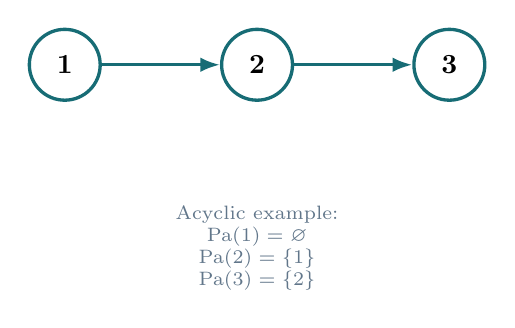
\begin{tikzpicture}[node distance=15mm]
\node[loc] (a) {1};
\node[loc,right=of a] (b) {2};
\node[loc,right=of b] (c) {3};
\draw[edge] (a)--(b);\draw[edge](b)--(c);
\node[note,below=12mm of b] {Acyclic example:\\ $\operatorname{Pa}(1)=\varnothing$\\ $\operatorname{Pa}(2)=\{1\}$\\ $\operatorname{Pa}(3)=\{2\}$};
\end{tikzpicture}
\par\vspace{6mm}
{\small\color{Muted}This is the same scalar SDM, not a new multivariate model.}
\end{columns}
\end{frame}

\begin{frame}{Each node is Gaussian given its parents}
Isolate the disturbance in the equation of location $i$:
\[
\varepsilon_i=y_i-\rho\sum_{j\in\operatorname{Pa}(i)}w_{ij}y_j
 -\beta x_i-\theta\sum_{j=1}^{3}w_{ij}x_j.
\]
Fix the parent outcomes and $x$. Then only $\varepsilon_i\sim N(0,\sigma^2)$ is random, and adding fixed numbers to it moves only its mean:
\[
\boxed{y_i\given(y_{\operatorname{Pa}(i)},x)\sim
 N\!\left(\rho\sum_{j\in\operatorname{Pa}(i)}w_{ij}y_j
 +\beta x_i+\theta\sum_jw_{ij}x_j,\,\sigma^2\right).}
\]
\smallnote{Acyclic: the nodes can be ordered so that every parent comes before its child. Each $\varepsilon_i$ is new at node $i$, so it is independent of the earlier nodes.}
\end{frame}

\begin{frame}{The joint density is a product over nodes}
\[
\boxed{p(y_1,y_2,y_3\given x)=\prod_{i=1}^3p(y_i\given y_{\operatorname{Pa}(i)},x).}
\]
Concrete case, the chain $1\to2\to3$ ($\operatorname{Pa}(1)=\varnothing$, $\operatorname{Pa}(2)=\{1\}$, $\operatorname{Pa}(3)=\{2\}$):
\begin{alignat*}{2}
p(y_1,y_2,y_3\given x)&=p(y_1\given x)\,p(y_2\given y_1,x)\,p(y_3\given y_1,y_2,x) &\qquad&\why{chain rule of probability (always true)}\\
&=p(y_1\given x)\,p(y_2\given y_1,x)\,p(y_3\given y_2,x) &&\why{$y_3$ is made from $y_2$, $x$, $\varepsilon_3$ only}
\end{alignat*}
Once $y_2$ and $x$ are given, $y_1$ does not change the distribution of $y_3$:
\keybox{y_1\indep y_3\given(y_2,x).}
\smallnote{This is the independence that SGS finds in Example 1.}
\end{frame}

\begin{frame}{D-separation: noncollider versus collider}
\small
\textbf{d-separation} is the rule that reads from the arrows alone which conditional independences every distribution on the DAG must have.
\vspace{1mm}
\begin{columns}[T,totalwidth=\linewidth]
\column{.49\linewidth}
\centering
\textbf{Noncollider path}\\[2mm]
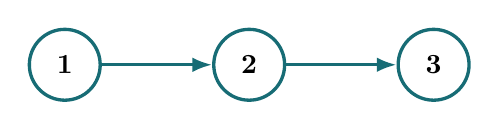
\begin{tikzpicture}[node distance=14mm]
\node[loc](a){1};\node[loc,right=of a](b){2};\node[loc,right=of b](c){3};
\draw[edge](a)--(b);\draw[edge](b)--(c);
\end{tikzpicture}
\[y_1\not\indep y_3\given x,\qquad\boxed{y_1\indep y_3\given(y_2,x)}\]
$\{2\}$ separates 1 and 3.\\ Conditioning on 2 blocks the path.
\column{.49\linewidth}
\centering
\textbf{Collider}\\[2mm]
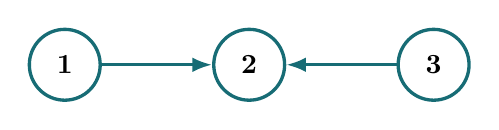
\begin{tikzpicture}[node distance=14mm]
\node[loc](a){1};\node[loc,right=of a](b){2};\node[loc,right=of b](c){3};
\draw[edge](a)--(b);\draw[edge](c)--(b);
\end{tikzpicture}
\[\boxed{y_1\indep y_3\given x},\qquad y_1\not\indep y_3\given(y_2,x)\]
$\varnothing$ separates 1 and 3.\\ Conditioning on the common effect 2 opens the path.
\end{columns}
\vspace{3mm}
SGS orients a collider \emph{only} when the middle node was not in the separating set.
\end{frame}

\begin{frame}{Acyclic does not mean uniquely orientable}
\centering
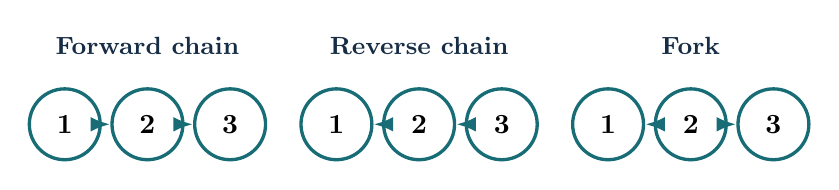
\begin{tikzpicture}[x=1.0cm,y=1cm]
\node[font=\small\bfseries,text=Navy] at (1.05,1.0) {Forward chain};
\node[loc](a1) at (0,0) {1};\node[loc](b1) at (1.05,0) {2};\node[loc](c1) at (2.10,0) {3};
\draw[edge](a1)--(b1);\draw[edge](b1)--(c1);
\node[font=\small\bfseries,text=Navy] at (4.5,1.0) {Reverse chain};
\node[loc](a2) at (3.45,0) {1};\node[loc](b2) at (4.5,0) {2};\node[loc](c2) at (5.55,0) {3};
\draw[edge](b2)--(a2);\draw[edge](c2)--(b2);
\node[font=\small\bfseries,text=Navy] at (7.95,1.0) {Fork};
\node[loc](a3) at (6.90,0) {1};\node[loc](b3) at (7.95,0) {2};\node[loc](c3) at (9.0,0) {3};
\draw[edge](b3)--(a3);\draw[edge](b3)--(c3);
\end{tikzpicture}
\par\vspace{5mm}
All three imply the same observed independence pattern:
\[y_1\indep y_3\given (y_2,x),\qquad y_1\not\indep y_3\given x.\]
\keybox{\text{Population SGS returns the same unoriented path }1-2-3.}
\smallnote{DAGs that imply the same conditional independences are called Markov equivalent.}
\end{frame}

\section{Worked examples}
\begin{frame}{Example 1: forward chain, $1\to2\to3$}
\begin{columns}[T,totalwidth=\linewidth]
\column{.34\linewidth}
\[W=\begin{pmatrix}0&0&0\\1&0&0\\0&1&0\end{pmatrix}\]
\begin{center}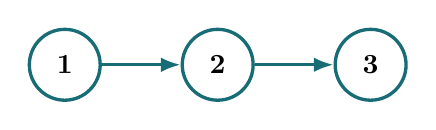
\begin{tikzpicture}[node distance=10mm]
\node[loc](a){1};\node[loc,right=of a](b){2};\node[loc,right=of b](c){3};
\draw[edge](a)--(b);\draw[edge](b)--(c);
\end{tikzpicture}\end{center}
\column{.62\linewidth}
Centering the outcomes ($\yt=y-\E[y\given x]$) gives:
\begin{alignat*}{2}
\yt_1&=\varepsilon_1 &\quad&\why{no parents}\\
\yt_2&=\rho\yt_1+\varepsilon_2=\rho\varepsilon_1+\varepsilon_2 &&\why{insert $\yt_1$}\\
\yt_3&=\rho\yt_2+\varepsilon_3=\rho^2\varepsilon_1+\rho\varepsilon_2+\varepsilon_3 &&\why{insert $\yt_2$}
\end{alignat*}
\end{columns}
\vspace{2mm}
\textbf{Before computing:} $\yt_1$ and $\yt_3$ share $\varepsilon_1$, so they are marginally dependent. Given $\yt_2$, the rest of $\yt_3$ is $\varepsilon_3$, which is independent of $\yt_1=\varepsilon_1$. So we expect $y_1\indep y_3\given(y_2,x)$.
\smallnote{The covariate and Durbin terms vanish from the centered equations because $x$ is fixed.}
\end{frame}

\begin{frame}{Example 1: compute covariance and delete $1-3$}
\small
Shared-disturbance rule, with $\yt_1=\varepsilon_1$, $\yt_2=\rho\varepsilon_1+\varepsilon_2$, $\yt_3=\rho^2\varepsilon_1+\rho\varepsilon_2+\varepsilon_3$:
\[
\Sigma_{13}=\rho^2\sigma^2,\quad
\Sigma_{12}=\rho\sigma^2,\quad
\Sigma_{23}=(\rho+\rho^3)\sigma^2,\quad
\Sigma_{22}=(1+\rho^2)\sigma^2.
\]
\begin{alignat*}{2}
\Cov(y_1,y_3\given y_2,x)
&=\Sigma_{13}-\frac{\Sigma_{12}\Sigma_{23}}{\Sigma_{22}} &\qquad&\why{conditional covariance formula}\\
&=\rho^2\sigma^2-\frac{(\rho\sigma^2)(\rho+\rho^3)\sigma^2}{(1+\rho^2)\sigma^2} &&\why{insert the four entries}\\
&=\rho^2\sigma^2-\frac{\rho^2(1+\rho^2)\sigma^2}{1+\rho^2}=\rho^2\sigma^2-\rho^2\sigma^2=\boxed{0} &&\why{$\rho(\rho+\rho^3)=\rho^2(1+\rho^2)$; cancel}
\end{alignat*}
\begin{block}{SGS on the originals}
Remove $1-3$. Keep $1-2$ and $2-3$: directly linked, $\Omega_{12}=\Omega_{23}=-\rho/\sigma^2\ne0$. The separating set $\{2\}$ contains the middle node: \emph{no} collider.
\end{block}
\end{frame}

\begin{frame}{Example 2: reverse chain, $1\leftarrow2\leftarrow3$}
\begin{columns}[T,totalwidth=\linewidth]
\column{.36\linewidth}
\[
W=\begin{pmatrix}0&1&0\\0&0&1\\0&0&0\end{pmatrix}
\]
\begin{center}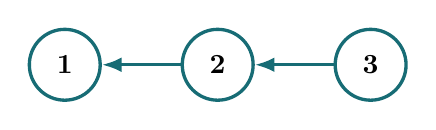
\begin{tikzpicture}[node distance=10mm]
\node[loc](a){1};\node[loc,right=of a](b){2};\node[loc,right=of b](c){3};
\draw[edge](b)--(a);\draw[edge](c)--(b);
\end{tikzpicture}\end{center}
\column{.60\linewidth}
\begin{alignat*}{2}
\yt_3&=\varepsilon_3 &\quad&\why{no parents}\\
\yt_2&=\rho\yt_3+\varepsilon_2=\rho\varepsilon_3+\varepsilon_2 &&\why{insert $\yt_3$}\\
\yt_1&=\rho\yt_2+\varepsilon_1=\varepsilon_1+\rho\varepsilon_2+\rho^2\varepsilon_3 &&\why{insert $\yt_2$}
\end{alignat*}
\end{columns}
\[
\Sigma_{13}=\rho^2\sigma^2,\quad \Sigma_{12}=(\rho+\rho^3)\sigma^2,\quad \Sigma_{23}=\rho\sigma^2,\quad \Sigma_{22}=(1+\rho^2)\sigma^2.
\]
\[
\Cov(y_1,y_3\given y_2,x)=\Sigma_{13}-\frac{\Sigma_{12}\Sigma_{23}}{\Sigma_{22}}=\rho^2\sigma^2-
\frac{(\rho+\rho^3)\sigma^2\cdot\rho\sigma^2}{(1+\rho^2)\sigma^2}=0.
\]
Given $\yt_2$, the rest of $\yt_1$ is $\varepsilon_1$, which is independent of $\yt_3=\varepsilon_3$. \good{SGS still returns the unoriented path $1-2-3$.}
\end{frame}

\begin{frame}{Example 3: fork, $1\leftarrow2\to3$}
\begin{columns}[T,totalwidth=\linewidth]
\column{.35\linewidth}
\[W=\begin{pmatrix}0&1&0\\0&0&0\\0&1&0\end{pmatrix}\]
\begin{center}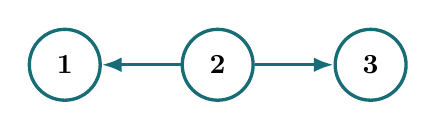
\begin{tikzpicture}[node distance=10mm]
\node[loc](a){1};\node[loc,right=of a](b){2};\node[loc,right=of b](c){3};
\draw[edge](b)--(a);\draw[edge](b)--(c);
\end{tikzpicture}\end{center}
\column{.61\linewidth}
\[
\begin{aligned}
\yt_2&=\varepsilon_2,\\
\yt_1&=\rho\varepsilon_2+\varepsilon_1,\\
\yt_3&=\rho\varepsilon_2+\varepsilon_3.
\end{aligned}
\]
\[
\Sigma_{13}=\rho^2\sigma^2,\quad\Sigma_{12}=\Sigma_{23}=\rho\sigma^2,\quad\Sigma_{22}=\sigma^2.
\]
\end{columns}
\[
\Cov(y_1,y_3\given y_2,x)=\Sigma_{13}-\frac{\Sigma_{12}\Sigma_{23}}{\Sigma_{22}}=\rho^2\sigma^2-\frac{(\rho\sigma^2)^2}{\sigma^2}=0.
\]
$\yt_1$ and $\yt_3$ share $\varepsilon_2$, so they are marginally dependent. Given $\yt_2=\varepsilon_2$, the rests $\varepsilon_1$ and $\varepsilon_3$ are independent. \good{Again SGS returns the unoriented path $1-2-3$.}
\end{frame}

\begin{frame}{Example 4: collider, $1\to2\leftarrow3$}
\begin{columns}[T,totalwidth=\linewidth]
\column{.35\linewidth}
\[W=\begin{pmatrix}0&0&0\\1&0&1\\0&0&0\end{pmatrix}\]
\begin{center}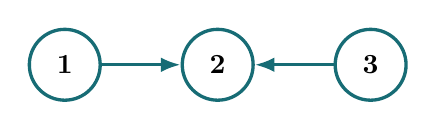
\begin{tikzpicture}[node distance=10mm]
\node[loc](a){1};\node[loc,right=of a](b){2};\node[loc,right=of b](c){3};
\draw[edge](a)--(b);\draw[edge](c)--(b);
\end{tikzpicture}\end{center}
\column{.61\linewidth}
\[
\begin{aligned}
\yt_1&=\varepsilon_1,\\
\yt_3&=\varepsilon_3,\\
\yt_2&=\rho\varepsilon_1+\varepsilon_2+\rho\varepsilon_3.
\end{aligned}
\]
\[
\Sigma_{13}=0,\quad\Sigma_{12}=\Sigma_{23}=\rho\sigma^2,
\quad\Sigma_{22}=(1+2\rho^2)\sigma^2.
\]
\end{columns}
\vspace{2mm}
$\yt_1=\varepsilon_1$ and $\yt_3=\varepsilon_3$ share no disturbance, so $\Sigma_{13}=0$.\\[1mm]
SGS removes $1-3$ \emph{without conditioning on 2}. This is the key collider signature.
\end{frame}

\begin{frame}{Example 4: conditioning on a collider creates dependence}
\small
With $\Sigma_{13}=0$, $\Sigma_{12}=\Sigma_{23}=\rho\sigma^2$, $\Sigma_{22}=(1+2\rho^2)\sigma^2$:
\begin{alignat*}{2}
\Cov(y_1,y_3\given y_2,x)
&=\Sigma_{13}-\frac{\Sigma_{12}\Sigma_{23}}{\Sigma_{22}} &\qquad&\why{conditional covariance formula}\\
&=0-\frac{(\rho\sigma^2)(\rho\sigma^2)}{(1+2\rho^2)\sigma^2} &&\why{insert the four entries}\\
&=\boxed{-\frac{\rho^2\sigma^2}{1+2\rho^2}\ne0}.
\end{alignat*}
\begin{block}{Why the sign is negative}
$\yt_2=\rho\varepsilon_1+\varepsilon_2+\rho\varepsilon_3$. Hold $\yt_2$ fixed. If $\yt_1=\varepsilon_1$ is large, then $\varepsilon_2+\rho\varepsilon_3$ must be smaller to keep $\yt_2$ fixed, so $\yt_3=\varepsilon_3$ tends to be smaller.
\end{block}
\textbf{Separating set for 1 and 3:} $\varnothing$, which does not contain node 2. Hence SGS orients the collider $1\to2\leftarrow3$.
\end{frame}

\begin{frame}{Example 5: reciprocal spatial feedback is not a DAG}
\begin{columns}[T,totalwidth=\linewidth]
\column{.46\linewidth}
\[
W=\begin{pmatrix}
0&1&0\\ \frac12&0&\frac12\\ 0&1&0
\end{pmatrix},\qquad 0<\rho<1.
\]
\begin{center}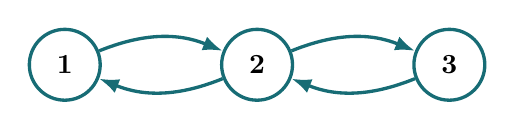
\begin{tikzpicture}[node distance=15mm]
\node[loc](a){1};\node[loc,right=of a](b){2};\node[loc,right=of b](c){3};
\draw[edge,bend left=22](a)to(b);\draw[edge,bend left=22](b)to(a);
\draw[edge,bend left=22](b)to(c);\draw[edge,bend left=22](c)to(b);
\end{tikzpicture}\end{center}
\column{.50\linewidth}
\begin{itemize}\setlength{\itemsep}{3mm}
\item $w_{13}=w_{31}=0$: no direct $1\leftrightarrow3$ weight.
\item $W$ contains two patterns at once:\\ \textbf{fork part} $1\leftarrow2\to3$ ($w_{12}=w_{32}=1$),\\ \textbf{collider part} $1\to2\leftarrow3$ ($w_{21}=w_{23}=\tfrac12$).
\item The system has directed cycles; it is \emph{not} a DAG-SEM on these nodes.
\end{itemize}
\end{columns}
\end{frame}

\begin{frame}{Example 5: even $1-3$ survives the SGS tests}
\small
From $\Omega=\frac1{\sigma^2}(I-\rho W)^{\mathsf T}(I-\rho W)$,
\[
\Omega=\frac1{\sigma^2}
\begin{pmatrix}
1+\rho^2/4 & -3\rho/2 & \rho^2/4\\
-3\rho/2 & 1+2\rho^2 & -3\rho/2\\
\rho^2/4 & -3\rho/2 & 1+\rho^2/4
\end{pmatrix}.
\]
\begin{columns}[T,totalwidth=\linewidth]
\column{.49\linewidth}
\textbf{Conditional test fails} (collider part):
\[\Omega_{13}=\frac{\rho^2w_{21}w_{23}}{\sigma^2}=\frac{\rho^2}{4\sigma^2}\ne0.\]
Location 2's equation contains both $y_1$ and $y_3$.
\column{.49\linewidth}
\textbf{Marginal test fails} (fork part):\\[1mm]
$\varepsilon_2$ enters both $\yt_1$ and $\yt_3$, so $\Sigma_{13}\ne0$. All pairwise marginal covariances are nonzero for $0<\rho<1$.
\end{columns}
\begin{block}{SGS outcome}
Neither test removes $1-3$: a complete three-node skeleton (triangle), even though $W$ has no direct $1-3$ link.
\end{block}
\end{frame}

\section{Interpretation}
\begin{frame}{Summary: original versus exactly field-filtered SGS}
\centering
\small
\renewcommand{\arraystretch}{1.35}
\begin{tabular}{@{}p{.26\linewidth}p{.32\linewidth}p{.29\linewidth}@{}}
\toprule
SDM input pattern & SGS on original $y$ & SGS on filtered $z$\\ \midrule
Forward chain & Unoriented path $1-2-3$ & No edges\\
Reverse chain & Unoriented path $1-2-3$ & No edges\\
Fork & Unoriented path $1-2-3$ & No edges\\
Collider & $1\to2\leftarrow3$ & No edges\\
Reciprocal path & Complete triangle & No edges\\
\bottomrule
\end{tabular}
\par\vspace{6mm}
\good{The empty filtered skeleton follows from independent Gaussian disturbances and exact realized-field subtraction.}
\end{frame}

\begin{frame}{Six tests for all five original-outcome examples}
\centering
\footnotesize
\renewcommand{\arraystretch}{1.16}
\begin{tabular}{@{}lcccccc@{}}
\toprule
&\multicolumn{3}{c}{Marginal}&\multicolumn{3}{c}{Condition on third}\\
Case & $1,2$ & $1,3$ & $2,3$ & $1,2\given3$ & $1,3\given2$ & $2,3\given1$\\
\midrule
Forward chain & D & D & D & D & I & D\\
Reverse chain & D & D & D & D & I & D\\
Fork & D & D & D & D & I & D\\
Collider & D & I & D & D & D & D\\
Reciprocal path & D & D & D & D & D & D\\
\bottomrule
\end{tabular}
\par\vspace{2mm}
\begin{block}{Reading the table}
\textbf{I}: independent. \quad \textbf{D}: dependent. All tests condition on fixed $x$.\\
Marginal columns: zeros of $\Sigma$. Conditional columns: zeros of $\Omega$.\\
For the exactly filtered $z$, all six entries are \textbf{I}.
\end{block}
\end{frame}

\begin{frame}{Realized field versus expected field}
\small
\textbf{Exact (realized) field removal:} $\ \boxed{y-f=\beta x+\varepsilon,\qquad\Cov(y-f\given x)=\sigma^2I.}$
\vspace{1mm}

\textbf{Expected field removal:} once $x$ is fixed, $\E[f\given x]$ is a fixed vector. Subtracting a fixed vector moves only the mean: $\ \boxed{\Cov(y-\E[f\given x]\given x)=\Cov(y\given x)=\Sigma.}$
\vspace{1mm}

Explicitly:\vspace{-2mm}
\begin{alignat*}{2}
y-\E[f\given x]&=\beta x+(f-\E[f\given x])+\varepsilon &\qquad&\why{$y=\beta x+f+\varepsilon$}\\
&=\beta x+\rho W\yt+\varepsilon &&\why{$f-\E[f\given x]=\rho W(y-\E[y\given x])=\rho W\yt$}\\
&=\beta x+\yt &&\why{$\varepsilon=(I-\rho W)\yt=\yt-\rho W\yt$}
\end{alignat*}
\begin{block}{Different operations, different SGS results}
The realized field contains the neighbours' actual disturbances, so subtracting it removes them. The expected field contains only their averages, so the mixing $\yt=(I-\rho W)^{-1}\varepsilon$ stays, with its original conditional-independence structure.
\end{block}
\end{frame}

\begin{frame}{Why the clean result need not hold in practice}
\begin{enumerate}\setlength{\itemsep}{4mm}
\item \textbf{Correlated structural errors:}
 $\Cov(z\given x)=\Cov(\varepsilon\given x)$ need not be diagonal.
\item \textbf{Random covariates with unconditional SGS:}
 $\Cov(z_i,z_j)=\beta^2\Cov(x_i,x_j)$ if $x\indep\varepsilon$ and errors are mutually independent.
\item \textbf{Estimated filters:} insert $\widehat\rho,\widehat\theta$ in place of $\rho,\theta$:
\[\widehat z=y-\widehat\rho Wy-\widehat\theta Wx=\beta x+\varepsilon+(\rho-\widehat\rho)Wy+(\theta-\widehat\theta)Wx.\]
The term $(\rho-\widehat\rho)Wy$ puts some of the neighbours' disturbances back.
\item \textbf{Reciprocal dependence:} a simultaneous SDM does not supply the same causal DAG as an acyclic SEM.
\end{enumerate}
\end{frame}

\begin{frame}{A defensible small-network empirical design}
\small
\begin{enumerate}\setlength{\itemsep}{2mm}
\item Fix the three locations, the same covariate, and a stable repeated-sampling design.
\item Specify the directed/reciprocal $W$ and row-normalization convention.
\item Separate the ideal known-parameter filter from the estimated filter.
\item Report all six independence checks, not only the final graph.
\item Compare skeletons and compelled collider arrows separately.
\item Diagnose sampling error, model assumptions, and faithfulness before causal claims.
\end{enumerate}
\vspace{1mm}
\begin{block}{Sampling warning}
One cross-section of three locations is one realization of $(y_1,y_2,y_3)$, not a sample large enough for SGS covariance tests.
\end{block}
\end{frame}

\begin{frame}{Conclusion}
\small
\begin{enumerate}\setlength{\itemsep}{2.5mm}
\item Exact removal of the \emph{realized} SDM field gives $z=\beta x+\varepsilon$.
\item With fixed $x$ and independent Gaussian errors, the filtered values share no disturbance, so population SGS on $z$ returns an \textbf{empty skeleton}.
\item SGS on the original $y$ can return an unoriented path, a compelled collider, or a triangle (fork part and collider part together).
\item Chain and fork orientations are \textbf{not} distinguished by observational conditional independence.
\item A sparser filtered graph is not automatically a more accurate causal graph.
\end{enumerate}
\vspace{0mm}
\keybox{\text{Filtering changes the statistical question SGS answers.}}
\end{frame}

\begin{frame}{Selected references}
\small
\begin{thebibliography}{5}
\bibitem{lesage} LeSage, J., and R. K. Pace (2009). \emph{Introduction to Spatial Econometrics}. Chapman \& Hall/CRC.
\bibitem{spirtes} Spirtes, P., C. Glymour, and R. Scheines (2000). \emph{Causation, Prediction, and Search}, 2nd ed. MIT Press.
\bibitem{verma} Verma, T., and J. Pearl (1990). ``Equivalence and Synthesis of Causal Models.'' UAI.
\bibitem{koller} Koller, D., and N. Friedman (2009). \emph{Probabilistic Graphical Models}. MIT Press.
\bibitem{peters} Peters, J., D. Janzing, and B. Sch\"olkopf (2017). \emph{Elements of Causal Inference}. MIT Press.
\end{thebibliography}
\end{frame}

\appendix
\section{Technical appendix}
\begin{frame}{Appendix: chain covariance matrix}
For $1\to2\to3$, using $\yt_1=\varepsilon_1$, $\yt_2=\rho\varepsilon_1+\varepsilon_2$, and $\yt_3=\rho^2\varepsilon_1+\rho\varepsilon_2+\varepsilon_3$:
\[
\Sigma=\sigma^2\begin{pmatrix}
1&\rho&\rho^2\\
\rho&1+\rho^2&\rho+\rho^3\\
\rho^2&\rho+\rho^3&1+\rho^2+\rho^4
\end{pmatrix}.
\]
\vspace{4mm}
$\Omega_{12}=\Omega_{23}=-\rho/\sigma^2\ne0$, but $\Omega_{13}=0$.
\smallnote{The conditional SGS checks preserve adjacent pairs and remove 1--3.}
\end{frame}

\begin{frame}{Appendix: collider covariance and precision}
For $1\to2\leftarrow3$:
\begin{align*}
\Sigma&=\sigma^2\begin{pmatrix}
1&\rho&0\\\rho&1+2\rho^2&\rho\\0&\rho&1
\end{pmatrix},\\
\Omega&=\frac1{\sigma^2}\begin{pmatrix}
1+\rho^2&-\rho&\rho^2\\-\rho&1&-\rho\\\rho^2&-\rho&1+\rho^2
\end{pmatrix}.
\end{align*}
The zero $\Sigma_{13}$ removes $1-3$ marginally; nonzero $\Omega_{13}$ means conditioning on 2 induces dependence.
\end{frame}

\begin{frame}{Appendix: why $\Omega_{ij}$ tests conditional independence}
\footnotesize
The inverse of a matrix is its cofactor matrix, transposed, divided by its determinant. For the pair $(1,3)$ given $2$: delete row 3 and column 1 of $\Sigma$.
\begin{alignat*}{2}
\Omega_{13}&=\frac{1}{\det\Sigma}\det\begin{pmatrix}\Sigma_{12}&\Sigma_{13}\\\Sigma_{22}&\Sigma_{23}\end{pmatrix} &\qquad&\why{cofactor formula for the inverse}\\
&=\frac{\Sigma_{12}\Sigma_{23}-\Sigma_{13}\Sigma_{22}}{\det\Sigma} &&\why{$2\times2$ determinant}\\
&=-\frac{\Sigma_{22}}{\det\Sigma}\left(\Sigma_{13}-\frac{\Sigma_{12}\Sigma_{23}}{\Sigma_{22}}\right) &&\why{factor out $-\Sigma_{22}$}\\
&=\boxed{-\frac{\Sigma_{22}}{\det\Sigma}\Cov(y_1,y_3\given y_2,x)} &&\why{conditional covariance formula}
\end{alignat*}
$\Sigma$ is positive definite, so $\Sigma_{22}>0$ and $\det\Sigma>0$. Hence $\Omega_{13}=0\iff\Cov(y_1,y_3\given y_2,x)=0$. The pairs $(1,2)$ and $(2,3)$ work the same way.
\smallnote{$\Omega_{ij}$ and the conditional covariance have opposite signs. Collider check: $\Omega_{13}=\rho^2/\sigma^2>0$ while $\Cov(y_1,y_3\given y_2,x)<0$.}
\end{frame}

\begin{frame}{Appendix: reciprocal feedback algebra}
\footnotesize
The centered simultaneous equations are
\[
\yt_1=\rho\yt_2+\varepsilon_1,\quad
\yt_2=\frac\rho2(\yt_1+\yt_3)+\varepsilon_2,\quad
\yt_3=\rho\yt_2+\varepsilon_3.
\]
\begin{alignat*}{2}
\yt_2&=\frac\rho2\big[(\rho\yt_2+\varepsilon_1)+(\rho\yt_2+\varepsilon_3)\big]+\varepsilon_2 &\qquad&\why{insert $\yt_1$ and $\yt_3$ into the middle equation}\\
(1-\rho^2)\yt_2&=\frac\rho2\varepsilon_1+\varepsilon_2+\frac\rho2\varepsilon_3 &&\why{move $\rho^2\yt_2$ to the left}\\
\yt_2&=\frac{\rho\varepsilon_1/2+\varepsilon_2+\rho\varepsilon_3/2}{1-\rho^2} &&\why{divide by $1-\rho^2>0$}\\
\yt_1&=\rho\yt_2+\varepsilon_1=\frac{(1-\rho^2/2)\varepsilon_1+\rho\varepsilon_2+(\rho^2/2)\varepsilon_3}{1-\rho^2} &&\why{insert $\yt_2$; common denominator}\\
\yt_3&=\frac{(\rho^2/2)\varepsilon_1+\rho\varepsilon_2+(1-\rho^2/2)\varepsilon_3}{1-\rho^2} &&\why{same steps, by symmetry}
\end{alignat*}
\smallnote{All three contain $\varepsilon_2$ (the fork part), so every marginal covariance is nonzero.}
\end{frame}

\begin{frame}{Appendix: feedback conditional covariance}
\footnotesize
Shared-disturbance rule on the three mixes above, with $d=1-\rho^2$:
\[
\Sigma_{13}=\frac{\sigma^2(2\rho^2-\rho^4/2)}{d^2},\qquad
\Sigma_{12}=\Sigma_{23}=\frac{3\rho\sigma^2}{2d^2},\qquad
\Sigma_{22}=\frac{(1+\rho^2/2)\sigma^2}{d^2}.
\]
\begin{alignat*}{2}
\Cov(y_1,y_3\given y_2,x)
&=\Sigma_{13}-\frac{\Sigma_{12}\Sigma_{23}}{\Sigma_{22}} &\qquad&\why{conditional covariance formula}\\
&=\frac{\sigma^2}{d^2}\left[2\rho^2-\frac{\rho^4}{2}-\frac{9\rho^2/4}{1+\rho^2/2}\right] &&\why{insert; the factor $\sigma^2/d^2$ is common}\\
&=\frac{\sigma^2}{d^2}\cdot\frac{-\frac{\rho^2}{4}+\frac{\rho^4}{2}-\frac{\rho^6}{4}}{1+\rho^2/2} &&\why{common denominator; expand}\\
&=\frac{\sigma^2}{d^2}\cdot\frac{-\frac{\rho^2}{4}(1-\rho^2)^2}{1+\rho^2/2} &&\why{$1-2\rho^2+\rho^4=(1-\rho^2)^2=d^2$}\\
&=\boxed{-\frac{\rho^2\sigma^2}{4(1+\rho^2/2)}\ne0} &&\why{cancel $d^2$}
\end{alignat*}
\end{frame}

\begin{frame}{Appendix: why a three-node DAG gives a finite inverse}
An acyclic three-node spatial-weights matrix with zero diagonal has $W^3=0$: a directed path with three arrows would need four distinct nodes.
\begin{alignat*}{2}
&(I-\rho W)(I+\rho W+\rho^2W^2) &&\\
&\quad=I+\rho W+\rho^2W^2-\rho W-\rho^2W^2-\rho^3W^3 &\qquad&\why{multiply out}\\
&\quad=I-\rho^3W^3=I &&\why{$W^3=0$}
\end{alignat*}
Thus the reduced form in the acyclic examples can be written without an infinite series:
\[
\boxed{(I-\rho W)^{-1}=I+\rho W+\rho^2W^2.}
\]
The $W^2$ term carries dependence along two-arrow paths. This matrix is the mixing table of the acyclic examples.
\end{frame}

\end{document}
